\section{System Architecture}\label{sec:architecture}

\begin{figure*}[t]
    \centering
    \begin{subfigure}[t]{0.7\textwidth}
        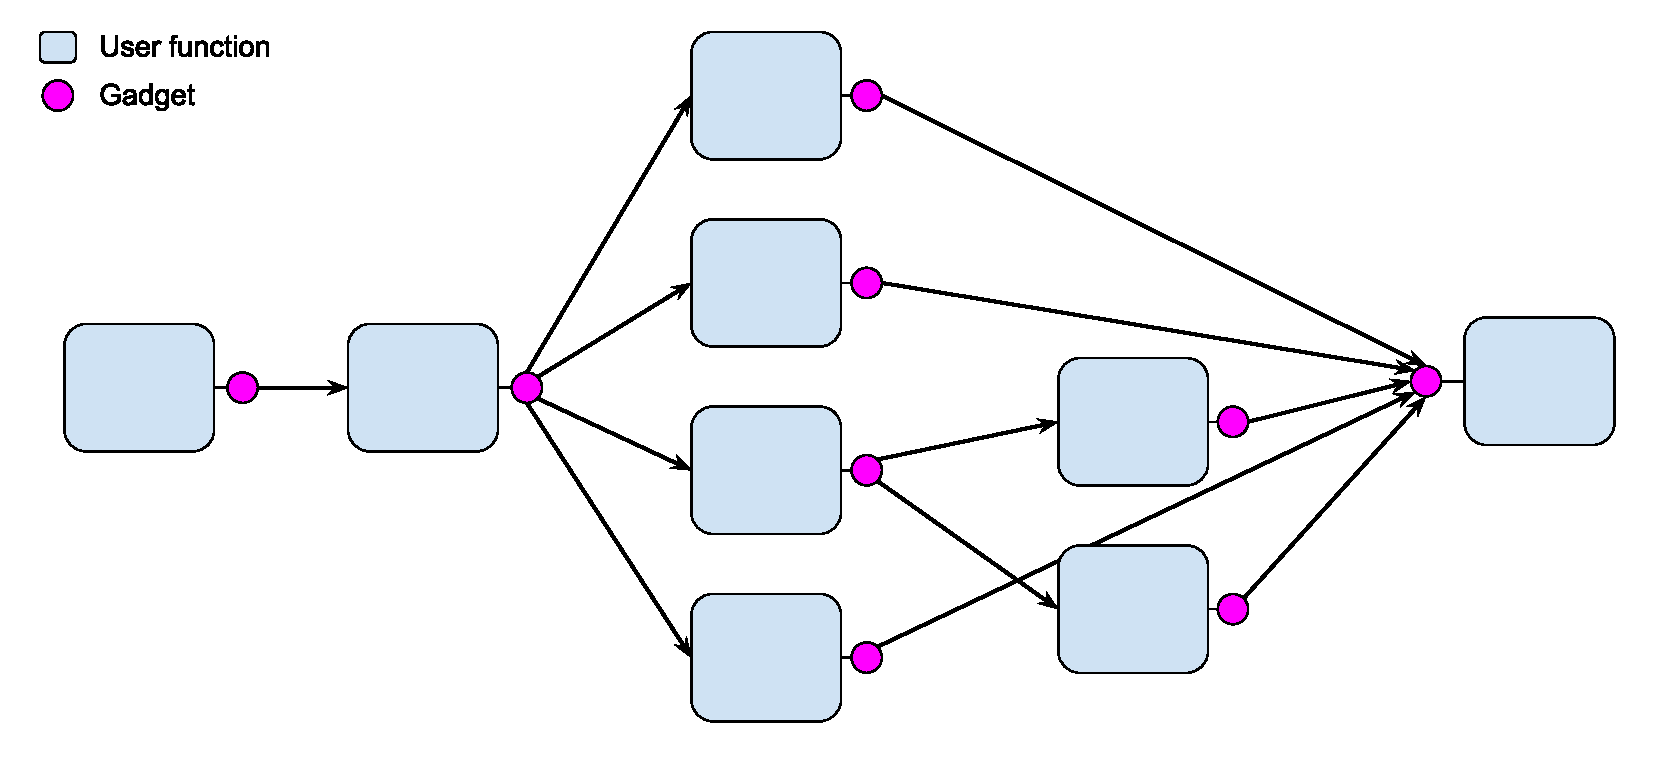
\includegraphics[width=\columnwidth]{figures/arch-abstract-graph.pdf}
        \caption{Stateful serverless computations form a directed graph. Nodes
                are user defined FaaS functions and workflow ``gadgets'' that dictate the
                communication pattern between user functions.}
        \label{fig:arch:graph}
    \end{subfigure}
    \begin{subfigure}[b]{\columnwidth}
        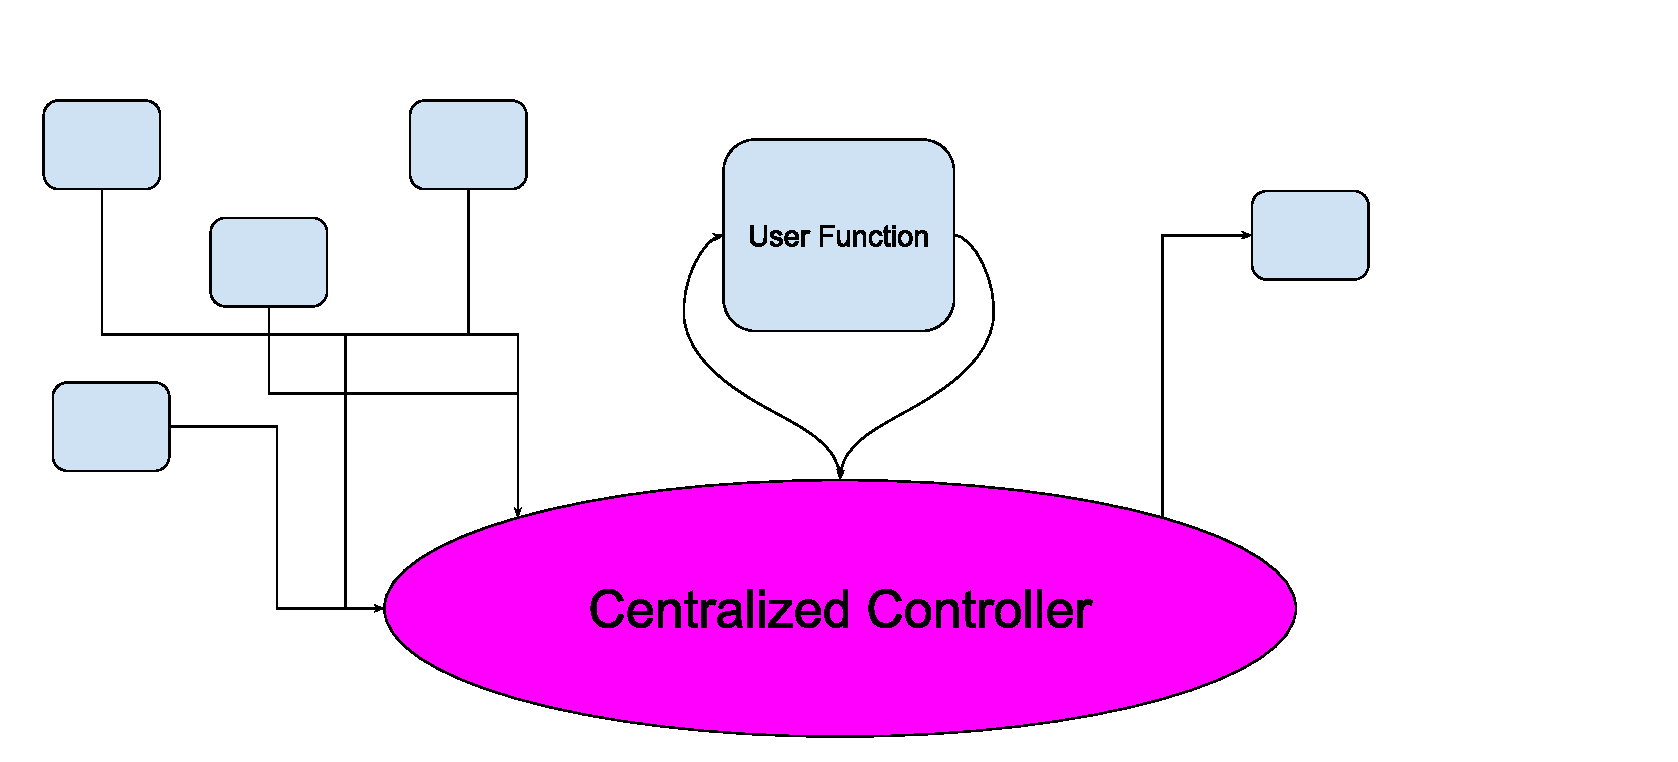
\includegraphics[width=\columnwidth]{figures/arch-controller.pdf}
        \caption{A typical stateful serverless system drives workflow logic
                 using a centralized controller that manages the computation's state-machine.}
        \label{fig:arch:centralized}
    \end{subfigure}
    \hfill
    \begin{subfigure}[b]{\columnwidth}
        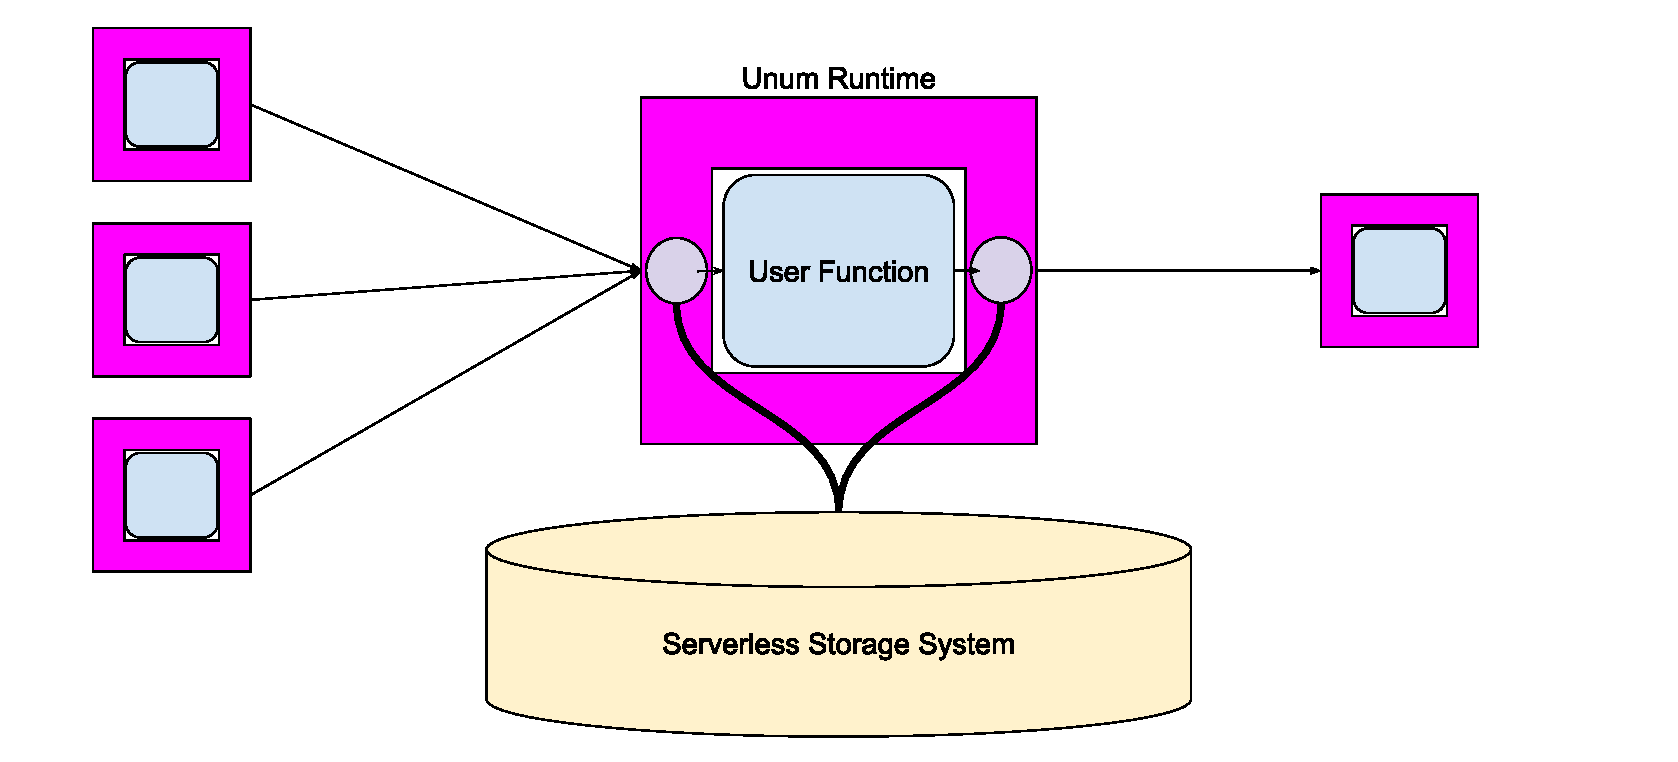
\includegraphics[width=\columnwidth]{figures/arch-system.pdf}
        \caption{\name{} decentralizes controller logic by running local state
                 transitions alongside Faas functions inside the \name{} runtime
                library. There is no centralized controller, instead \name{} relies on existing
                serverless datastores such as DynamoDB or Cosmos DB.}
        \label{fig:arch:unum}
    \end{subfigure}
    \caption{\name{} System Overview. Serverless computations form a directed
            graph that encode sequential and data dependencies between functions. Workflow
            orchestrators drive these graphs by centralizing control flow logic and
            interposing on all communication between functions. \name{},
            instead, decentralizes control flow logic among the functions with
            no need for a separate orchestration system.}
    \label{fig:arch}
\end{figure*}

Computations are a directed graph connecting ``simple'' stateless functions
using, potentially, stateful workflow patterns, such as chaining, map, fan-out,
and fan-in. Existing systems implement stateful patterns by centralizing
control-flow state in an orchestrator. Figure~\ref{fig:arch} contrasts this with
\name{}'s decentralized approach.

\name{} introduces no new components that run separately from basic serverless
infrastructure.  Instead, \name{} encompasses a runtime library that implements
decentralized workflow logic, an intermediate representation to describe
workflow control logic, and front-end compilers to transform high-level workflow
representations written by developers to the intermediate representation.

TODO: gadgets are the secret sauce, in particular noticing that fan-in needs to
be split between the source and target functions \emph{and} that source
functions must coordinate.

Developers write workflows using high-level description languages, such as AWS
Step Functions or Google Workflows. An \name{} front-end compiler transforms
this high-level description to \name{}'s intermediate representation (IR), and
embeds portions of the control-flow logic to appropriate functions. Control-flow
in the IR is encoded as ``gadgets''---platform-independent control-flow patterns
that can be implemented efficiently in a decentralized manner. Finally, the
developer combines their functions with a platform-specific \name{} runtime
which implements gadgets using platform-specific APIs and datastores.

TODO: gadgets don't run where programmers express them. Example with fan-in.
This is kind of the ``magic'' of the front-end compiler.

\section{Gadgets}\label{sec:gadgets}

A key challenge in designing a decentralized workflow orchestrator is
determining where to store control-flow state and where to execute
state-transitions. \name{} uses the notion of a gadget---a special kind node in
the control-flow graph that can implement complex interaction patterns using any
datastore and FaaS API that adheres to the requirements in
Section~\ref{sec:motivation}.

Logically, every user-defined function in \name{} has exactly one input and one
output edge---it is invoked once with a single value and outputs its result to
at most one node. This makes user functions simple to program and allows \name{}
to embed complex platform-specific orchestration logic in gadgets implemented by
the runtime.

\name{} provides four gadgets that map can express a rich variety of workflows
efficiently, including a superset of workflows expressible in Step Functions.
Each user function outputs has an outgoing edge to a gadget and fan-in targets,
with multiple incoming edges, are combined into a single edge by a fan-in
specific gadget which outputs a single edge to the target user function.

Table~\ref{tab:gadgets} lists the gadgets available in \name{}.  At
compile-time, \name{} injects these gadgets into the nearest function and
executes them in the \name{} runtime that wraps the function. Thus there is no
system overhead for running the gadgets---they are, effectively, embedded in
the functions themselves.

\begin{table}[t!]
  \centering
  \begin{tabular}{ |m{8em}| m{13em} | }
    \hline
      \texttt{chain(a,b) }& Invokes function \texttt{b} with the output of \texttt{a} \\
    \hline
      \texttt{fanOut(a, [b])} & Invokes each element of \texttt{[b]} with the output from \texttt{a} \\
    \hline
      \texttt{map(a, b)} & Invokes \texttt{b} once for each element in the vector output of \texttt{a} \\
    \hline
      \texttt{fanIn([a], b)} & Invokes \texttt{b} once with the vector of outputs from each of \texttt{[a]} \\
    \hline
\end{tabular}
  \caption{\name{} workflows express complex interactions using a small set of gadgets.} 
  \label{tab:gadgets}
\end{table}

\paragraph{Chain}
Chaining is a simple but common interaction. For example, an application might
include a function that processes input data from a sensor followed by another
function that makes a control decision based on the processed input. The
\texttt{chain} gadget connects two user functions together by invoking one
function with the result of another. At runtime, \name{} uses the platform's
asynchronous function invocation API to call the target function directly from
the source, without requiring any additional storage interactions.


\paragraph{Fan-out}
Another common interaction processes the output of a function in different ways
in parallel. For example, an application might perform several independent
functions given a new user post, such as URL shortening and resolving other
users mentioned in th post. The \texttt{fanOut} gadget invokes the a vector of
functions each with the output from a previous function. Similar to chaining,
\name{} uses the function invocation API to simply invoke each of the target
functions from the source function directly. \amit{TODO: Are there special
considerations for exactly-once semantics? i.e. is checkpointing different than
it is in chaining?}

\paragraph{Map}
An application may also perform the same function on multiple outputs of a
source function. For example, a photo management application might unpack an
archive of high-resolution images in one function and perform compression or
down-scaling on each of the resulting images. The \texttt{map} gadget invokes
the same function once for each element in a vector of outputs from the
previous function. \amit{TODO: Are there special considerations for
exactly-once semantics? i.e. is checkpointing different than it is in
chaining?}

\amit{TODO: I feel like there is a bunch of complexity, particularly with
fan-in, do with assigning indexes to branches, etc, that is part of the
platform-agnostic design of unum, so should be here. But I don't recall the
specifics. Are there also similar things for the other gadgets?}

\paragraph{Fain-in}
Takes an scalar outputs from each fan-in branch and outputs a vector of
outputs the the fan-in target function. Each branch stores its output to the
datastore and performs an atomic operation on the datastore competing to see if
they are the last of the branches to complete. The last branch invokes the
fan-in target function passing it a vector of pointers to each of the branches
stored output. The fan-in function dereferences each of the pointers by reading
from the data store and passes a vector of output values to the target function.

% chain = invoke, fan-out = a bunch of invoke, one for each continuation;
% Additionally, in the case of Map, one invoke for each element of the array
% (output of the user function).  fan-in .... well.... let's see. The semantics
% is: invoke the fan-in function once when all of its inputs are ready. In
% practice, it is each branch synchronize over the data store to see if all
% branches have completed. The last branch to complete calls invoke on the fan-in
% function, and pass it pointers to all branches results/checkpoints in the data
% store. The fan-in function first reads the branches' results, in order, via the
% pointers, then pass them as input to the user code.

\section{Design}\label{sec:design}

% Notes(alevy):
%
% * Consider splitting design section into separate sections for System Architecture and IR/Language
% * Design needs to describe the (non)-architecture of unum. There are pieces of functionality that typically exist in a controller that still exist in unum, they are just embedded in
% unum runtime. Maybe we can give this 'component' a name, like a distributed controller (the unum runtime then implements the distributed controller).
% * The design includes too many implementation specific details, and doesn't really describe the high level operations. If the big question is 'how do you implement fan-out / fan-in
%   in a distributed way?', the section should answer that directly (same for other interactions which are much simpler).
% * Similarly, we need to describe the interactions that unum provides and sort of hand-wave argue that these are the right set of interactions (perhaps by pseudo-code example).
%
% Terms to use:
% * 'Gadgets': The interactions that are encoded in unum_config (fan-out, fan-in, chain, etc)
% * 'Execution graph': where nodes are either user-code (Lambda functions) or gadgets, edges exiting user-code always enter gadgets. Instead of talking about
%    continuations (I really don't think that Unum has something that looks like continuations), this execution graph is the IR and the runtime reifies the
%    execution graph by embedding gadgets in lambdas themselves.

%\begin{figure*}[t]
%    \centering
%    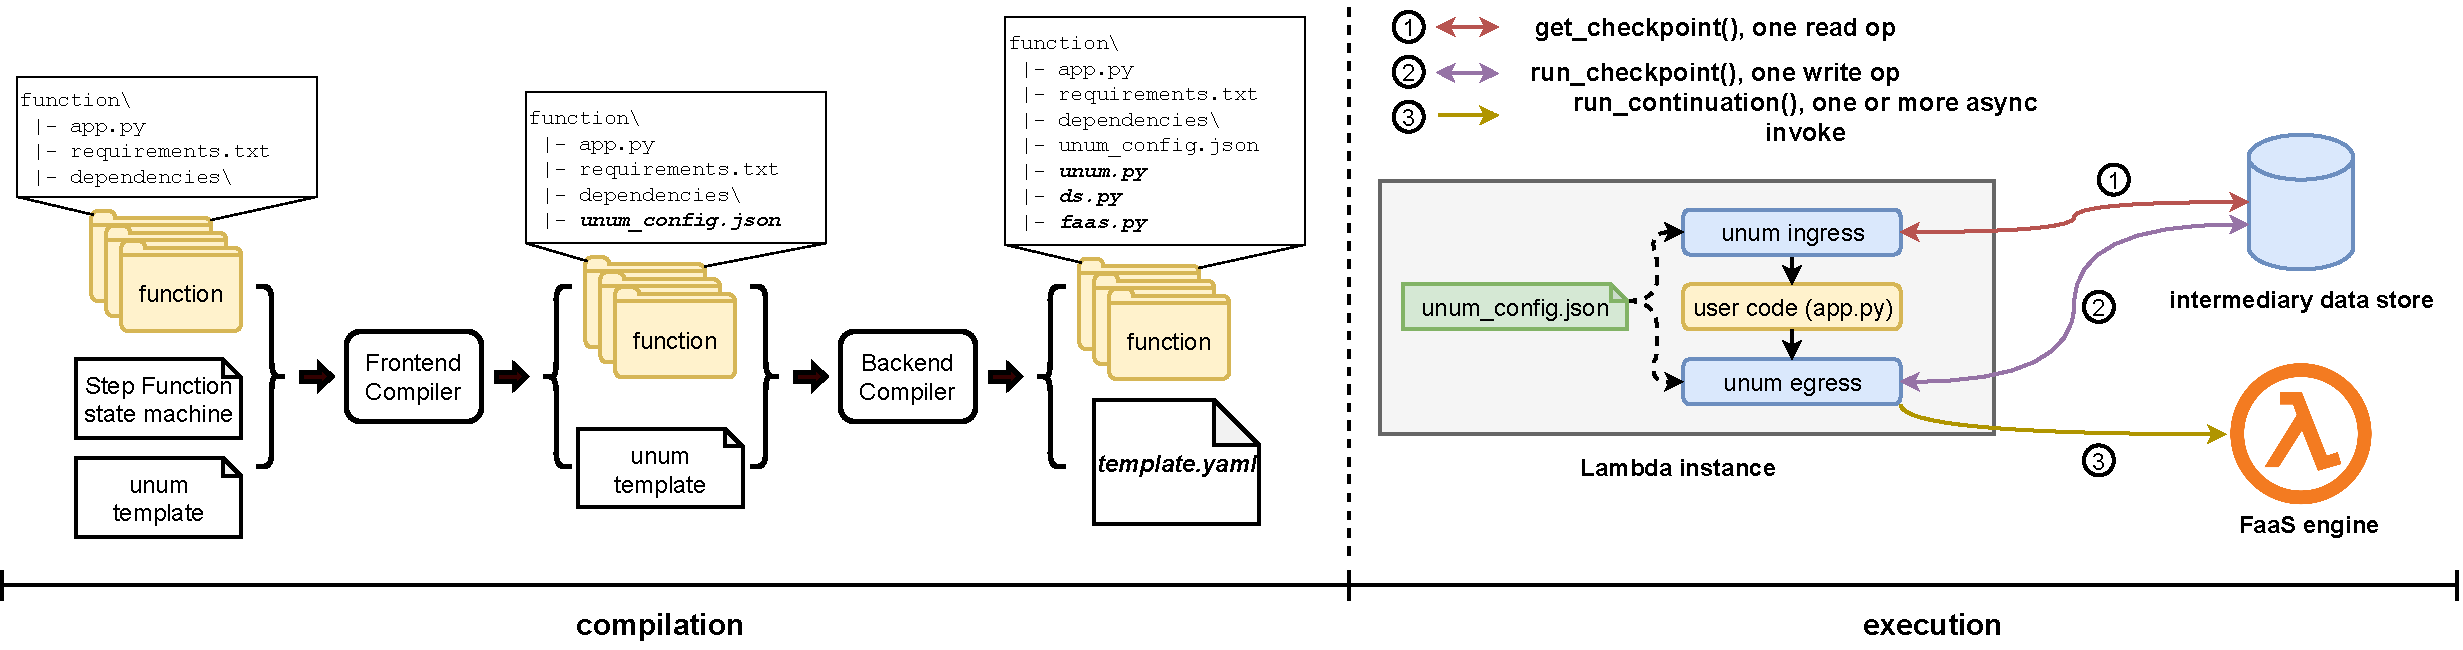
\includegraphics[width=\textwidth]{figures/unum-arch.pdf}
%    \caption{\name{}'s architecture}
%    \label{fig:arch}
%\end{figure*}

\begin{figure}[]
    \begin{minted}[
    frame=single,
    linenos,
    fontsize=\footnotesize
  ]{yaml}
Globals:
  ApplicationName: unum-iot-chain
  UnumIntermediaryDataStoreType: dynamodb
  UnumIntermediaryDataStoreName: iot-intermediary
  Checkpoint: true
  Debug: false
Functions:
  Aggregator:
    Properties:
      CodeUri: aggregator/
      Runtime: python3.8
      Start: true
  HvacController:
    Properties:
      CodeUri: hvac_controller/
      Runtime: python3.8
      Policies:
        - AmazonSQSFullAccess
  \end{minted}
    \caption{The unum template for an IoT HVAC controller
    application. It lists all resources of the workflow (Two functions:
    \texttt{Aggregator} and \texttt{HvacController}. A DynamoDB table
    \texttt{iot-intermediary} used as the intermediary data store) and
    specifies workflow-wide options such as checkpoint, debug and
    application name.}
    \label{fig:iot-unum-template}
\end{figure}


\begin{figure}[]
    \begin{minted}[
    frame=single,
    linenos,
    fontsize=\footnotesize
  ]{json}
{
  "StartAt": "Aggregator",
  "States": {
    "Aggregator": {
      "Type": "Task",
      "Resource": "Aggregator",
      "Next": "HvacController"
    },
    "HvacController": {
      "Type": "Task",
      "Resource": "HvacController",
      "End": true
    }
  }
}
    \end{minted}
    \caption{A Step Functions state machine for an IoT HVAC controller
    application. The workflow is a chain of two functions \texttt{Aggregator}
    and \texttt{HvacController}. When \texttt{Aggregator},
    \texttt{HvacController} should be invoked with \texttt{Aggregator}'s
    result. Note that normally the \texttt{"Resource"} fields are the deployed
    Lambda's ARN. Here they are function names defined in the unum template
    (see Figure~\ref{fig:iot-unum-template})}
    \label{fig:iot-sf}
\end{figure}

\begin{figure}[]
    \begin{minted}[
    frame=single,
    linenos,
    fontsize=\footnotesize
  ]{json}
{
    "Name": "string",
    "Next": {
        "Name": "FunctionName",
        "InputType": "Scalar" | "Map" | "Fan-in",
        "Condtional": "BooleanExpression"
    },
    "Next Payload Modifiers" : ["str"],
    "Checkpoint": "True | False",
    "Start": "True | False"
}
    \end{minted}
    \caption{}
    \label{fig:unum-config-lang}
\end{figure}

\begin{figure}[]
    \begin{minted}[
    frame=single,
    linenos,
    fontsize=\footnotesize
  ]{json}
{
    "Data": {
        "Source": "http | <data store type>",
        "Value": "<JSON object> | [<data store pointers>]"
    },
    "Session": "uuid",
	"Fan-out": {
        "Index": "int",
        "Size": "int",
        "OuterLoop": {
            "Index": "int",
            "Size": "int"
        }
    }
}
    \end{minted}
    \caption{}
    \label{fig:input-format}
\end{figure}

A key feature in \name{}'s approach is that it is designed as a runtime on top
of the serverless abstraction without requiring any supplemental services
added to current infrastructures. Workflows built with \name{} can execute in
any environment that has a FaaS engine with an asynchronous invocation API and
a named data store that supports strongly consistent reads. Both are readily
available on all existing serverless platforms.

Architecturally, \name{} eliminates the need for any specialized, hosted
processes that execute workflows, manage system states or broker
inter-function communication. FaaS functions are the only compute entity in
\name{} that runs code. They execute both user code and the \name{} runtime. The
\name{} runtime directly invokes the next function in the workflow after user
code completes and leverages a checkpointing mechanism to ensure strong
execution guarantees.

We continue this section by first giving an overview of unum's architecture
(\S~\ref{sec:design-overview}) and outlining the serverless abstractions and
services that \name{} builds upon (\S~\ref{sec:design-req}). We then
describe the programming interface that \name{} supports
(\S~\ref{sec:design-interface}). Next, we discuss the \name{} IR
(\S~\ref{sec:design-ir}) which expresses serverless workflows using
continuations. Finally, we describe \name{}'s runtime
(\S~\ref{sec:design-runtime}) and execution guarantees
(\S~\ref{sec:design-exec-gntee}).

\subsection{Overview}\label{sec:design-overview}

Figure~\ref{fig:arch} illustrates \name{}'s high-level architecture. At
compile-time, a frontend compiler transforms workflows written for existing
systems (e.g., an AWS Step Functions state machine that orchestrates Lambdas)
into a continuation-based, platform-independent intermediary representation.
In practice, the IR is a set of configuration files
(\texttt{unum\_config.json}), one for each function in the workflow, written
in the \name{} configuration language (\S~\ref{sec:design-config-lang}).

Next, a backend compiler compiles the IR into platform-specific packages that
are executable in a particular target environment (e.g., AWS Lambda with
DynamoDB as the data store). Deploying the packages will create a set of FaaS
functions (e.g., Lambdas) and an intermediary data store (e.g., a DynamoDB
table or S3 bucket).

A workflow is invoked by triggering the entry function. Each unum workflow has
one and only one entry function. \shadi{does it have to be one entry point? why?}

At execution time, each function runs both the user code and the unum runtime.
The unum runtime manages the function's checkpoint and invokes the
continuation asynchronously after user code completes. unum uses checkpoints
to provide strong execution guarantee. Every function invocation in unum is
assigned a unique name and the runtime uses the name for the instance's
checkpoint in the data store.

\subsection{System Requirements}\label{sec:design-req}

\name{} utilizes two services that are readily available on all existing
serverless platforms:

\begin{enumerate}

	\item A Function-as-a-Service engine that supports an
	\emph{asynchronous invocation API}.

	\item A shared data store that supports creating and reading items by
	 their unique names.

\end{enumerate}

\subsubsection{FaaS engine with asynchronous invocation}

Support for asynchronous invocation is universal across all major FaaS
engines, including AWS Lambda~\cite{aws-lambda-async-invoke}, Azure
Functions~\cite{azure-functions-async-invoke}, Google Cloud
Functions~\cite{google-cloud-functions-async-invoke}, and popular open-source
options such as OpenWhisk~\cite{openwhisk-async-invoke} and
OpenFaaS~\cite{openfaas-async-invoke}.

\name{} chooses asynchronous invocation because functions in \name{} directly invoke
their immediate downstream functions and asychronous invocation avoids
timeouts, and double billing. If only synchronous invocation is available, a
function has to idly wait for all of its downstream functions, immediate or
not, to complete, risking function timeouts and incurring double billing.

\paragraph{At-least-once invocation}

FaaS engines normally only guarantee at-least-once invocation of
asynchronously triggered
functions~\cite{google-cloud-functions-exec-guarantee,
aws-lambda-async-invoke, azure-functions-exec-guarantee}. A single invocation
might result in the FaaS engine running the same function more than once. Such
duplicate invocations are especially problematic when the function is
non-deterministic (i.e., given the same input, the function might produce
different output across runs) and all serverless providers simply urge
developers to write deterministic functions to avoid incorrect behavior.

From a workflow system's perspective, it has a few options to work with an
at-least-once FaaS engine: (1). it can equire all functions to be
deterministic (2). make sure functions are invoked exactly-once (3). ensure
that even if a non-deterministic function executes more than once, only one of
the results is taken as the final result and propagated to the rest of the
workflow.

\name{} takes the third approach as the first is restrictive and the second is
unattainable. \name{} uses a checkpointing mechanism to make sure only the
execution that finishes first is taken as the final result and propagated
downstream. Duplicates are simply discarded. We discuss the details in
\S~\ref{sec:design-runtime}.

\subsubsection{Named data store}

Functions in \name{} workflows use a named data store to store checkpoints and
other intermediary data (\S~\ref{sec:design-runtime}) during execution. The
data store needs to support creating and later retrieving objects with unique
names.

There is a wide variety of data store services that can support \name{}
workflows, including object storage (e.g., Amazon S3, AZure Blob Storage),
NoSQL databases (e.g., DynamoDB, Cosmos DB) and key-value stores (e.g.,
Redis).

Nearly all of the storage services above have a "serverless" option that
requires no explicit provisioning and users only pay for what they use.

\paragraph{Consistency Requirements}

\name{} requires the data store to be strongly consistent.

Strongly consistent reads (read that return the most up-to-date data,
reflecting all prior writes that were successful) are important for the
correctness of aggregations (e.g., fan-in), because it prevents the
possibility where all upstream functions have completed and written their
checkpoint but none of them sees that all have completed and thus never invoke
the fan-in function.

Note that strong consistency alone is not enough for correct execution of
aggregation patterns because multiple functions might detect that all fan-out
branches have completed and thus invoking the fan-in functions more than once.
\name{} runtime contains additional synchronization logic to make sure the fan-in
function is only invoked once. We discuss the details in
\S~\ref{sec:design-runtime}


\subsection{Programming Interface}\label{sec:design-interface}

\name{} does not introduce a new programming interface for building serverless
workflows. Developers can use familiar frontend languages from existing
systems, such as the Amazon State Language for AWS Step Functions.

Moreover, \name{} lets developers write component functions in
workflows exactly the same way as they would for regular functions. In fact,
orchestration-related logic are entirely transparent from user functions'
perspective. There is no additional libraries that user code needs to import
or use.

Figure~\ref{fig:arch} gives an example of using Step Functions state machine
to define the workflow that orchestrates functions in Python. Each
function is defined in its own directory with the exact same content as you
would have for regular functions that are not part of any workflow.

The \emph{unum template} is a YAML file that lists all the resources in the
workflow and specifies workflow-wide configurations.
Figure~\ref{fig:iot-unum-template} gives an example of an IoT HVAC controller
application's template.

The frontend compiler transforms the workflow definition to a
continuation-based, platform-independent intermediary representation (IR)
which we discuss in the next section.



\subsection{\name{} IR}\label{sec:design-ir}

The \name{} intermediary representation expresses FaaS workflows using
continuations. A continuation defines (1). which function(s) to invoke (2).
what input to invoke it with.

After running user code, the unum runtime invokes the continuation with the
user code's result as the input. Every function in a unum workflow has 0, 1 or
more continuations. The set of continuations from all functions form the
complete workflow.

unum continuations form graphs with functions as vertices. They support common
orchestration patterns such as chaining, branching, fan-out and fan-in. unum
also supports \texttt{for} or \texttt{while} loop (fold) with continuation
graphs that have directed cycles.

A key benefit of the continuation-based IR is to distribute workflows'
orchestration logic to individual component functions so that it can execute
without a centralized orchestrator. In an orchestrator-based workflow system,
functions will need to call back to the orchestrator service to signal
completion and it is the orchestrator who will then invoke the next function.

In contrast, unum assigns each function a set of continuations \emph{at
compile-time}. After user code completes, each function directly invokes its
continuations asynchronously, without involving any supplemental services.

% \subsubsection{Naming scheme}

% \name{} assigns each function instance a unique name. The name consists of the
% function's name and, if the instance is part of a fan-out, the instance's
% fan-out index.



\subsubsection{\name{} configuration language}\label{sec:design-config-lang}

In practice, the \name{} IR is a set of configuration files (by default named
\texttt{unum\_config.json}), one for each function in the workflow, written in
the \name{} configuration language.

Figure~\ref{fig:patterns} shows 2 examples patterns and how to express them in
the \name{} IR.

The configuration language provides constructs to define continuations. Each
continuation is a JSON object. It specifies the name of the function to invoke
(the \texttt{"Name"} field), what its inputs are (the \texttt{"InputType"}
field) and an invoke condition (the \texttt{"Conditional"} field).

The function name needs to match one of the names in the \name{} template. The 

Continuations are defined in the \texttt{"Next"} field. The value is
either a single JSON object if there is only one continuation or an array
of JSON objects if there are multiple continuations.

% Figure~\ref{fig:iot-sf} shows a Step Functions state machine for an IoT HVAC
% controller workflow which is a chain of two functions. Figure~\ref{fig:iot-ir}
% shows the generated IR in the form of two \texttt{unum\_config.json} files.

\begin{itemize}

	\item Every function has a \texttt{unum\_config.json} file deployed with
	it.

	\item Continuations are defined in the \texttt{"Next"} field. The value is
	either a single JSON object if there is only one continuation or an array
	of JSON objects if there are multiple continuations.

	\item Each continuation is a JSON object. It specifies the name of the
	function to invoke next in the \texttt{"Name"} field, what its inputs are
	in the \texttt{"InputType"} field and an invoke condition in the
	"Conditional" field.

	\item \texttt{"InputType"} has three possible values: \texttt{"Scalar"},
	\texttt{"Map"} and \texttt{"Fan-in"}.

	\item \texttt{"Scalar"} is used when the only input to the next function
	is the output of this function.

	\item \texttt{"Scalar"} supports chaining, where the input to the next
	function is the output of the previous function, and fan-out, where
	multiple functions are triggered in parallel with the output of the
	previous function.

	\item Give example \texttt{unum\_config.json} files of chaining and
	fan-out with \texttt{"Scalar"}?

	\item \texttt{"Map"} supports a different form of fan-out where the output
	of this function is an array and for each element of the array, the
	runtime invokes one instance of the next function with the element as
	input.

	\item \texttt{"Fan-in"} is used for aggregations when the next function to
	invoke depends not only on the result of this function but also on those
	of other functions. (Give a concrete example here?)

	\item Values that the next function depends on are listed in the
	\texttt{"Values"} field. Each value is identified by the unique name of
	the function instance that produces it. We discuss \name{}'s naming scheme
	in the next section.

	\item Value names can include glob patterns to support fan-in of varying
	size. unum expands glob patterns during runtime.

	\item The "Conditional" field is a boolean expression. Only when the
	boolean expression evaluate to Ture would the continuation be invoked.

	\item Workflow entry functions have \texttt{"Start: true"}.

	\item "Next Payload Modifiers" is an interface to modify \name{}'s runtime
	metadata. 

\end{itemize}


\subsection{Runtime}\label{sec:design-runtime}

\begin{itemize}

	\item \name{}'s runtime interposes on user code's entry and exit (See
	Figure~\ref{fig:arch}. On ingress, \name{} runtime reads the input data
	and then pass it to user code. When user code returns, the egress takes
	the return value, write it to the data store as a checkpoint and invokes
	the continuation.

	\item Inputs to unum functions are JSON objects.
	Figure~\ref{fig:input-format} shows the input format.

	\item \texttt{"Data"} field contains the input data to the user code. If
	the data is directly sent in the function invocation via HTTP (i.e.,
	\texttt{"Source": "http"}), the value of the "Value" field is passed to
	user code unchanged. If the \texttt{"Source"} field shows that the data is
	in the intermediary data store (e.g., \texttt{"Source": "dynamodb"}),
	\name{} reads the data from the data store and then pass it to user code.

	\item In practice, \name{} only passes data via the data store in the case
	of fan-in where results of multiple functions are needed. In that case,
	the \texttt{"Value"} field is an array of names of function checkpoints.
	\name{} reads each checkpoint in the array in order and passes the data as
	an array to user code.

	\item User code is oblivious of the \name{} runtime. \name{} does not
	change how user code is written or its interface.

	\item \texttt{"Session"} field contains a UUID string that uniquely
	identifies a workflow invocation. \name{} runtime on the entry function
	creates the UUID string when the function is invoked. The string
	propagates to all downstreams function instances that are part of the
	workflow invocation.

	\item Checkpoint names are prefixed with the \texttt{"Session"} UUID
	string so that instances of the same function from different invocations
	do not overwrite each others' results.

	\item "Fan-out" field are part of fan-out functions' input payload.
	\name{} assigns each fan-out function an index.

	\item \name{} supports nested fan-outs with the \texttt{"OuterLoop"} field
	that is recursive.

	\item Each function instance is assigned a unique name. The name consists
	of the function's name and, if the function is part of a fan-out, its
	fan-out indexes. Example?

	\item Fan-in semantics. Only invoke the continuation once when all inputs
	are ready. For data stores with atomic data structures, we use them to
	synchronize. For data stores without atomic data structures, \name{}
	pre-select that last function in the \texttt{"Value"} array to wait for
	all other functions to complete.

\end{itemize}

% \subsubsection{Checkpoints?}


% check checkpoint existence before running user function

% run user function or read from existing checkpoint

% write checkpoint or pass

% run continuation

% checkpoints are used both for guaranting execution correctness and for
% aggregation patterns such as fan-in.


\subsection{Fault tolerance and execution guarantee}\label{sec:design-exec-gntee}

Challenges to providing strong execution guarantees:

\begin{enumerate}

	\item Functions in the workflow can fail at any point.

	\item FaaS engines only provide at-least-once execution guarantee on
	individual functions. Triggering a function once might result in duplicate
	executions.

\end{enumerate}

Given the limitation of the underlying FaaS engines, \name{} cannot guarantee
exactly-once execution on \emph{individual functions}. However, \name{}
guarantees:

\begin{enumerate}

	\item At-least-once invocation on individual functions. This ensures that a
	workflow invocation will not just stuck somewhere and not proceed.

	\item In a particular workflow invocation, a particular function will
	always be invoked with the exact same input.

	\item Each workflow invocation will produce exactly one result. Even if
	there happen to be duplicate executions of functions, and even if the
	functions are non-deterministic, only a single result is recorded, while
	any duplicate and potentially diverging results are discarded.

\end{enumerate}

From users' perspective, if none of the functions in the workflow have
external side-effects (e.g., writing to external services), the workflow will
appear to execute exactly-once.

\name{} leverages the at-least-once execution guarantee of FaaS engines to
ensure that functions run at least once.

When a workflow execution crashes before finishing, \name{} only retries the
function where the crash happens instead of restarting the entire workflow.
\name{} leverages the automatic retry feature that most FaaS engines already provide
for individual functions~\cite{azure-functions-retry,
google-cloud-functions-retry, aws-lambda-async-invoke}.

\name{} uses checkpointing to make sure that even if a function executes more
than once, whether due to retries or duplicate invocations, only the result of
one of the executions is taken as the final result, and only the final result
is propagated downstream to the rest of the workflow.

\name{} checkpointing process is the following:

First, before running user code, the ingress checks to see if a checkpoint
already exists for the invocation. If it does, \name{} skips running user code
and uses the checkpoint's content as the result. The egress will invoke the
continuation again in case the prior execution crashed after checkpointing but
before running the continuation. This makes sure that if a step in the
workflow has completed and persisted, it will not run again.

If a checkpoint doesn't exist, unum runs the user code. After the user
function completes, unum checkpoints the result into the data store and runs
the continuation.
